\documentclass[11pt,oneside,a4paper,onecolumn]{report}
\usepackage{graphicx}
\usepackage{color}
\usepackage{setspace}
\usepackage{hyperref}
\usepackage{morefloats}
\usepackage{amsmath}
\usepackage{setspace}
\usepackage{subcaption}
\usepackage{enumitem}
\usepackage{bm} %allows for bold mathematical symbols (e.g. \bm{X})
\usepackage{siunitx} %correct typesetting for SI units (e.g. \SI{50}{\hertz})
%\singlespacing
\doublespacing
\usepackage[margin=1in]{geometry}
\setlength{\parindent}{20pt} % Do not automatically indent the paragraphs.

\newcommand{\SB}{SUPERball} %use \SB{} to write "SUPERball" correctly

\begin{document}

\title{DESIGN, BUILDING, AND TESTING OF \SB{}:\\ A TENSEGRITY ROBOT TO ENABLE SPACE EXPLORATION}
\author{Jonathan Bruce}

\maketitle


%%%%%%%%%%%%%%%%%%%%%%%%%%%%%%%%%%%%
%%% Begin Table of Contents Page
%%%%%%%%%%%%%%%%%%%%%%%%%%%%%%%%%%%%
\renewcommand\contentsname{Table of Contents} % This command changes the name of the autogenerated table of contents (next line) from "Contents" to "Table of Contents".
\tableofcontents % This command automatically generates the table of contents based on the sections in the document.
\pagebreak[4]

%%%%%%%%%%%%%%%%%%%%%%%%%%%%%%%%%%%%
%%% End Table of Contents Page
%%%%%%%%%%%%%%%%%%%%%%%%%%%%%%%%%%%%

%%%%%%%%%%%%%%%%%%%%%%%%%%%%%%%%%%%%
%%% Begin List of Figures Page
%%%%%%%%%%%%%%%%%%%%%%%%%%%%%%%%%%%%

\phantomsection % Create a phantom section such that the 'List of Figures' may be properly added to the table of contents.
\addcontentsline{toc}{section}{List of Figures} % Add this section, 'List of Figures', to the table of contents.
\listoffigures % This command automatically generates the list of figures based on the figures in the document.
\pagebreak[4]

%%%%%%%%%%%%%%%%%%%%%%%%%%%%%%%%%%%%
%%% End List of Figures Page
%%%%%%%%%%%%%%%%%%%%%%%%%%%%%%%%%%%%

%%%%%%%%%%%%%%%%%%%%%%%%%%%%%%%%%%%%
%%% Begin List of Tables Page
%%%%%%%%%%%%%%%%%%%%%%%%%%%%%%%%%%%%

\phantomsection % Create a phantom section such that the 'List of Tables' may be properly added to the table of contents.
\addcontentsline{toc}{section}{List of Tables} % Add this section, 'List of Tables', to the table of contents.
\listoftables % This command automatically generates the list of tables based on tables in the document.
\pagebreak[4]

%%%%%%%%%%%%%%%%%%%%%%%%%%%%%%%%%%%%
%%% End List of Tables Page
%%%%%%%%%%%%%%%%%%%%%%%%%%%%%%%%%%%%



\chapter{Introduction}
\begin{singlespace}
\emph{The text and ideas presented in this section were originally proposed by the NASA Innovative Advance Concepts (NIAC) solicitation submitted in 2013 and granted in 2014~\cite{NIACfinalreport}.
My dissertation proposal draws heavily from this project and was funded by this grant.}
\end{singlespace}

\section{Motivation}

\begin{figure}[htb]
   \centering
   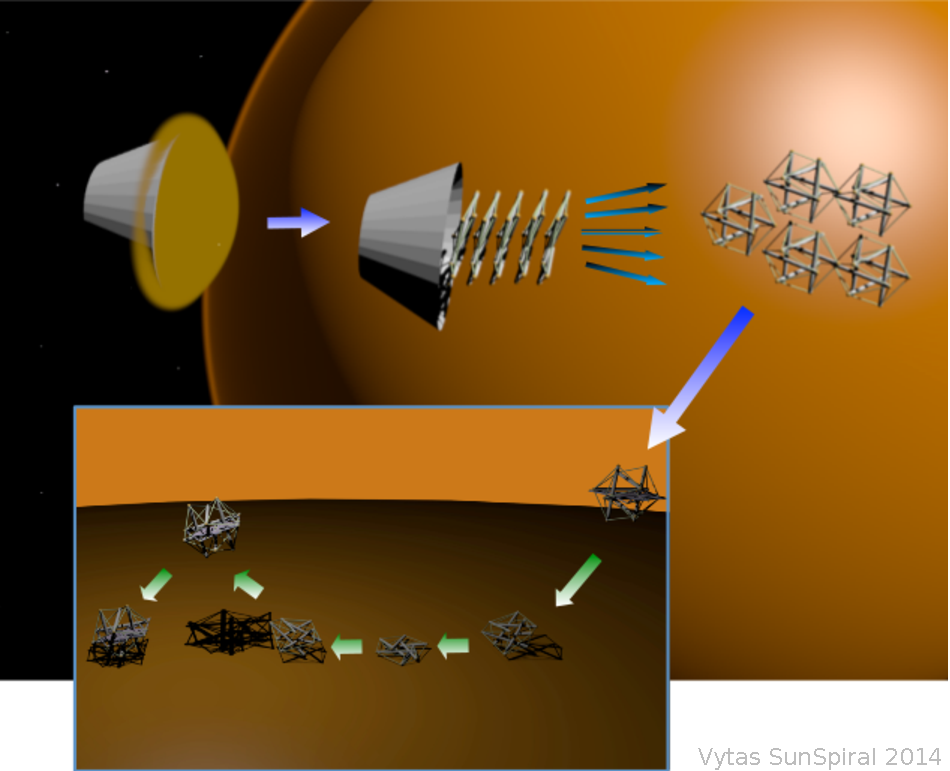
\includegraphics[width=0.5\textwidth]{tex/img/fig_aeroshell_summary} 
   \caption{{\em Tensegrity structures are composed of pure compression and tension elements. They can be lightweight, reliable, deployable, and efficient to manipulate. {\bf Mission Scenario} - Tightly packed set of tensegrities, expand, spread out, fall to surface of moon, then safely bounce on impact. The same tensegrity structure which cushioned the landing is then used for mobility to explore moons such as Titan and small asteroids.}}
   \label{fig:unpack}
\end{figure}

Tensegrity robots can facilitate an intriguing low-cost planetary exploration mission profile (see Figure~\ref{fig:unpack}) comprising of the following stages:  1) A set of tensegrity robots can be squeezed into a small launch platform; 2)  After initial atmospheric entry and ejection of the heat shield, they can automatically spring away from each other when released at their destination. 3) They ``bounce'' on impact reducing the need for final descent equipment, such as airbags; and 4) They can reorient themselves from landed position without addition reorientation hardware and efficiently move from scattered initial positions to perform sensor measurements; 5) They can survive significant falls and are resistant to being stuck, simplifying route planning and allowing for more aggressive exploration in the pursuit of science.

Once on the surface, tensegrity robots can perform an array of scientific analysis including soil and atmospheric composition, surface imagery and microscopic analysis. To further reduce complexity, sensors can be suspended on the interior of the tensegrity on cables attached to the nodes, or when appropriate even to the nodes themselves so that the sensors can be moved with movements of the structure itself, eliminating the need for separate sensor arms. In addition, environmental analysis can be performed in-situ at the landing site, at different local locations, or even at distant locations given a tensegrity robot's potential for efficient locomotion. The biggest advantages of this mission profile are:
\begin{enumerate}[leftmargin=.5cm]
\item The structure of the robot itself provides capability for deployment, landing (EDL), and mobility, reducing complexity, risk, and mass compared to using three separate systems.
\item Tensegrity robots are light-weight and can be packed tightly, reducing cost.
\item Can scale to multiple tightly packed robots to increase scientific coverage and reduce risk.
%TODO do we want to keep this statement on multiple robots?
\item Flexibility and modularity of robot design allows design reuse, reducing mission project risk.
\end{enumerate}

 \begin{figure}[h]
   \centering
   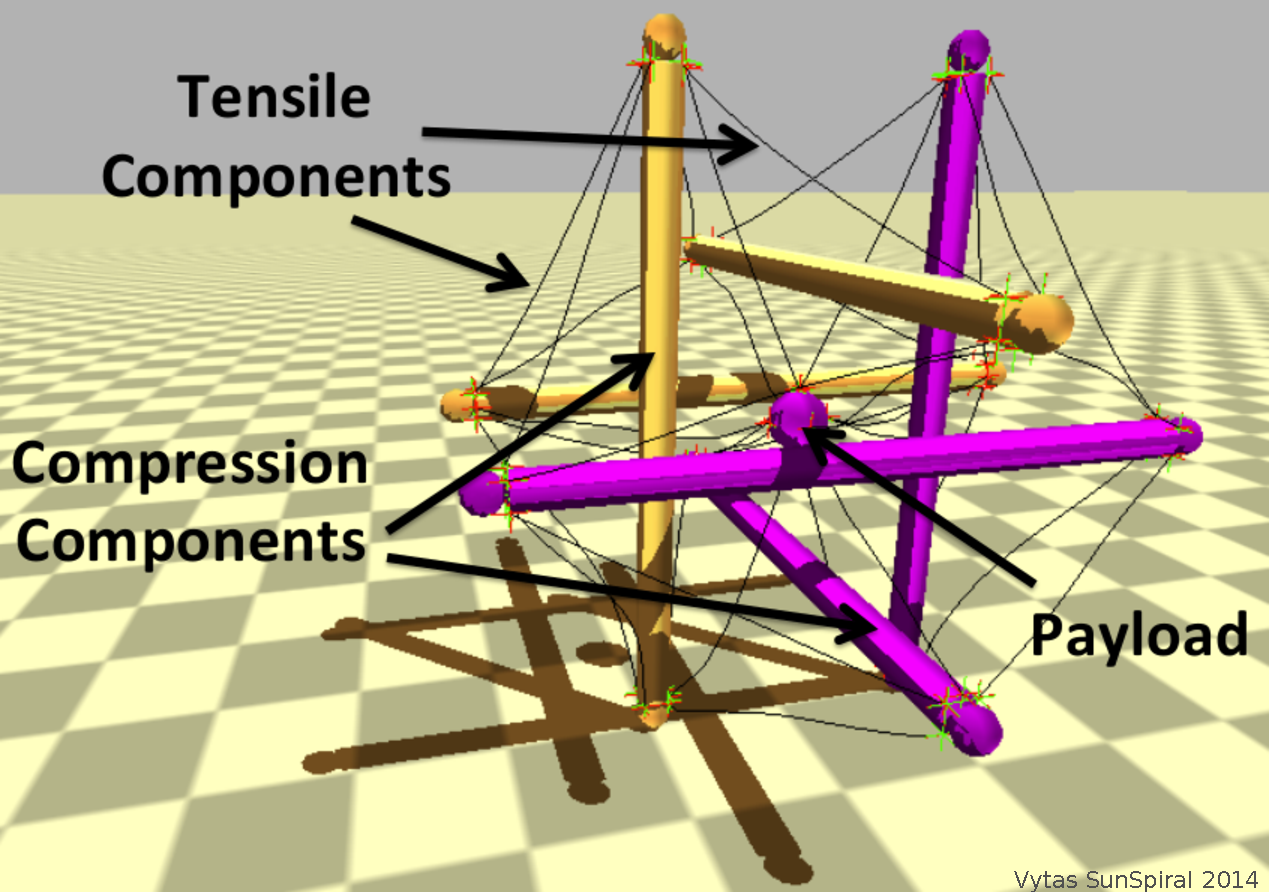
\includegraphics[width=0.5\columnwidth]{tex/img/fig_basic_diagram}
   \caption{{\em {\bf Tensegrity Structure.} Tensegrities are composed of pure tension and pure compression elements (e.g. cables and rods) as seen in this picture of a tensegrity robot from our physics based tensegrity simulator. They are light-weight, energy-efficient and robust to failures.}}
   \label{fig:basic_diagram1}
\end{figure}

\section{Goals}
\label{goal}
The main goals my project seeks to accomplish:

\begin{enumerate}[leftmargin=.5cm]
\item \textbf{Build a rolling tensegrity robot}\\
A physical hardware prototype of an untethered tensegrity robot to explore locomotion.
The robot will not only need to perform the basics for rolling, but will need to enable the next two goal items.
To achieve this, the robot will need significant mechanical power, distributed computation, and wireless communication.

\item \textbf{Open loop locomotion control}\\
Once the hardware prototype is built, an open loop control scheme will be developed.
The open loop algorithm will not change the control inputs to the system based on sensing outside of the robot.
This will demonstrate the system's ability to coordinate motion between it's distributed computation and collect data wirelessly.

\item \textbf{Closed loop "gait" control}\\
Once the system has proven the ability to locomote open loop, a closed loop algorithm will be developed.
The closed loop control will change the "gait", or locomotion pattern, of the robot to cope with sensed variations in terrain, e.g. changes in terrain grade or climbing over an obstacles.
To achieve this, research into the how much of the robot state is needed as well as various techniques to model and predict the environment by using the on board sensors.
\end{enumerate}

\chapter{Literature Review}

\section{Tensegrity Structures}
It is possible to design free-standing structures with axially loaded compression elements in a well crafted network of tensional elements.
Such an arrangement is called a tensegrity structure (tensile integrity). 
Each element of the structure experiences either pure axial compression or pure tension \cite{BuckminsterFuller1975}\cite{Snelson1965}.
The absence of bending or shear forces allows for highly efficient use of materials, 
resulting in lightweight, yet robust systems.

Because the struts are not directly connected, 
tensegrities have the unique property that externally applied forces distribute through the structure via multiple load paths. 
This creates a soft structure, for a soft robot, out of inherently rigid materials.
Since there are no rigid connections within the structure, there are also no lever arms to magnify forces. 
The result is a global level of robustness and tolerance to forces applied from any direction.

%Tensegrity structures are composed of axially loaded compression elements encompassed within a network of tensional elements, and thus each 
%element experiences either pure linear compression or pure tension.  As a result, individual elements can be extremely lightweight as there are no 
%bending or shear forces that must be resisted.  Because the struts are not directly connected, a unique property of tensegrity structures is how externally applied forces distribute through the structure 
%via multiple load paths, creating a system level robustness and tolerance to forces applied from any direction.  
%Because there are no rigid connections within the structure, there are also no lever arms to magnify forces.  Instead, all experienced forces act linearly on each structural element.  Combined with the ability to diffuse forces globally, 
This makes tensegrity robots inherently compliant and extremely well suited for physical interactions with complex and poorly modeled natural environments.  
Active motion in tensegrity robots can be performed by changing cable lengths in parallel, 
enabling the use of many small actuators that work together, rather than individual heavy actuators which work in series.  
There are also many indications that tensegrity properties are prevalent throughout biological systems, 
and the morphology of the SUPERball that we are studying, 
especially when carrying a payload, 
ends up bearing a striking resemblance to the nucleated tensegrity model of cell structure~\cite{Wang2009}\cite{Wang2001}.

\section{Prior Work in Tensegrity Robotics Design}
An important advantage of tensegrity structures with respect to general pin-jointed structures is their increased mass-efficiency due to a high fraction of tensile members.
Tensile members are generally more mass-efficient as they do not need to resist buckling.
A further advantage from a robotics perspective is that forces diffuse in a tensegrity.
There are no lever arms and torques do not accumulate at the joints as in a classic serial manipulator.
Forces distribute through multiple load paths, thus increasing robustness and tolerance to mechanical failure.

%advantages
%applications
The static properties of tensegrities have been thoroughly studied and some basic analysis is discussed in section \ref{modeling}.
On the other hand, few examples are known of truly dynamic motion of these structures.
Early examples of kinematic motion include the work at EPFL's IMAC laboratory~\cite{Fest2004}.
Skelton and Sultan introduced algorithms for the positioning of tensegrity based telescopes and the dynamic control of a tensegrity flight simulator platform~\cite{sultan2000tensegrity}.
Although there were some early efforts at MIT's CSAIL lab, it wasn't until the work of Paul and Lipson at Cornell University that the concept of tensegrity robotics became widespread~\cite{Paul2006a}.
Paul and Lipson were the first to study the properties of dynamic tensegrity structures in hardware and simulation.
A few years later Fivat and Lipson designed the IcoTens, a small actuated tensegrity icosahedron robot, but did not publish results.
In recent years, the BIER lab at the University of Virginia has been studying Central Pattern Generator based control for tensegrity based fish tails,
which is closely related to the control architectures proposed for SUPERball~\cite{Caluwaerts2013rsif,Bliss2012}.
Mirats-Tur has presented design and controls work on various other tensegrity morphologies that have been tethered or fixed to the ground~\cite{GraellsRovira2009,miratstur2011athree-dof}.
At Union College, Rieffel and colleagues are following an interesting line of work by considering vibration based actuation for small tensegrities~\cite{khazanov2014developing}.
Related work was presented by B\"ohm and Zimmermann, who demonstrated controlled locomotion of vibration driven tensegrity robots with a single actuator~\cite{bohm2013vibration}.
Finally, Shibata, Hirai and colleagues have developed pneumatically actuated rolling tensegrity structures~\cite{Shibata2009}. 
%goal

Building upon these works, the \SB{} project seeks to push forward the tensegrity robotics field and develop truly untethered, highly dynamic and compliant robots exploiting the aforementioned advantages.

\section{Tensegrity Robotics for Space Exploration}
%NASA is supporting research into tensegrity robotics to create robots with many of the same qualities that benefit biological systems.  
The high strength-to-weight ratio of tensegrity structures is very attractive due to the impact of mass on mission launch costs. 
Large tensegrity structures have been shown to be deployable from small compact configurations which enable them to fit into space constrained launch fairings.   
While the above qualities have inspired studies of deployable antennae and other large space structures~\cite{Tibert2002}, 
it is in the realm of planetary exploration that we see the most significant role for many of the unique force distribution qualities of tensegrity robots.  
The NIAC project currently funding this research~\cite{NIACfinalreport} specifically studies landing and surface mobility of tensegrities,
exploiting the controllable compliance and force distribution properties which make for reliable and robust environmental interactions.  

The main goal is to develop tensegrity probes with an actively controllable tensile network
 to enable compact stowage for launch, followed by deployment in preparation for landing. 
Due to their natural compliance and 
structural force distribution properties, tensegrity probes can safely absorb 
significant impact forces, enabling high speed Entry, Descent, and Landing 
(EDL) scenarios where the probe itself acts much like an airbag.  However, 
unlike an airbag which must be discarded after a single use, the tensegrity 
probe can actively control its shape to provide compliant rolling mobility 
while still maintaining the ability to safely absorb impact shocks that might 
occur during exploration.  This combination of functions from a single 
structure enables compact and lightweight planetary exploration missions 
with the capabilities of traditional wheeled rovers, but with a mass and 
cost similar or less than a stationary probe.   

Therefore, a large fraction of the overall weight (as measured at atmospheric entry) of a tensegrity mission can be used for the scientific payload 
due to the dual use of the structure as a lander and a rover. 
This allows for cheaper missions and enable new forms of surface exploration that utilize the natural tolerance to impacts of tensegrities~\cite{Vytas_IPPW_2013}.

% Because  of  the  limited  research  into  actuated  tensegrity
% robotics,   many   design   aspects   have   yet   to   be   carefully
% studied. To date, the majority of constructed tensegrity robots
% have  been  simple  prototypes  using  servo  motors,  limited
% sensing,  and  are  often  tethered  for  power  and  control  [5].
% Others have had fewer limbs than the SUPER ball, or have
% been  secured  to  the  ground  as  opposed  to  free-standing
% [6][7]. Some related approaches utilize tensegrity as part of a
% larger, more complicated system, but not as the primary loco-
% motion method [8]. Others have created designs that do not
% use direct cable actuation, as in the SUPER ball, but instead
% have  more  limited  forms  of  locomotion  through  vibration
% [9][10]. Finally, the most similar designs to the SUPER ball
% have not been engineered to specific design requirements nor
% have  the  advanced  sensing  framework  needed  for  controls
% testing [11]
%
% The  high  strength-to-weight  ratio  of  tensegrity  structures
% is very attractive due to the impact of mass on mission launch
% costs.  Large  tensegrity  structures  have  been  shown  to  be
% deployable from small compact configurations which enable
% them to fit into space constrained launch fairings. While the
% above qualities have inspired studies of deployable antennae
% and  other  large  space  structures  [12],  it  is  in  the  realm
% of  planetary  exploration  that  we  see  the  most  significant
% role  for  many  of  the  unique  force  distribution  qualities  of
% tensegrity  robots.  A  recent  NIAC  project  [13]  specifically
% studies  landing  and  surface  mobility  of  tensegrities,  ex-
% ploiting  the  controllable  compliance  and  force  distribution
% properties which make for reliable and robust environmental
% interactions.
% The   main   goal   is   to   develop   tensegrity   probes   with
% an  actively  controllable  tensile  network  to  enable  compact
% stowage  for  launch,  followed  by  deployment  in  preparation
% for  landing.  Due  to  their  natural  compliance  and  structural
% force  distribution  properties,  tensegrity  probes  can  safely
% absorb significant impact forces, enabling high speed Entry,
% Descent, and Landing (EDL) scenarios where the probe itself
% acts  much  like  an  airbag.  However,  unlike  an  airbag  which
% must  be  discarded  after  a  single  use,  the  tensegrity  probe
% can  actively  control  its  shape  to  provide  compliant  rolling
% mobility  while  still  maintaining  the  ability  to  safely  absorb
% impact  shocks  that  might  occur  during  exploration.  This
% combination  of  functions  from  a  single  structure  enables
% compact and lightweight planetary exploration missions with
% the capabilities of traditional wheeled rovers, but with a mass
% and cost similar or less than a stationary probe.
%
% Therefore, a large fraction of the overall weight (as mea-
% sured  at  atmospheric  entry)  of  a  tensegrity  mission  can  be
% used  for  the  scientific  payload  due  to  the  dual  use  of  the
% structure  as  a  lander  and  a  rover.  This  allows  for  cheaper
% missions  and  enable  new  forms  of  surface  exploration  that
% utilize the natural tolerance to impacts of tensegrities [14].
%
% Buckminster Fuller [1] and the artist Kenneth Snelson [2]
% initially  explored  tensegrity  structures  in  the  1960s.  Until
% the  mid-1990s  the  majority  of  tensegrity  related  research
% was  concerned  with  form-finding  [15]  and  design  analysis
% of  static  structure  [16][17].  More  recently,  active  control
% efforts  for  tensegrities  began  to  emerge  [18],  as  well  as
% descriptions  of  the  dynamics  of  tensegrity  structures  taking
% the connectivity pattern into account [17].
% The tensegrity principle allows for compliance and multi-
% path load distribution, which is ideal for physical interaction
% with  the  environment.  However,  these  aspects  also  present
% significant  challenges  to  traditional  control  approaches.  A
% recent  review  [19]  shows  that  there  are  still  many  open
% problems in actively controlling tensegrities, especially when
% interacting  with  an  environment  during  locomotion  or  ma-
% nipulation  tasks.  Though  work  has  been  done  to  control  a
% tensegrity  to  change  into  a  specified  shape  [20],  practical
% determination  of  the  desired  shape  itself  is  an  ongoing
% challenge.  Recently,  locomotion  of  icosahedral  tensegrity
% robots  through  body  deformation  was  demonstrated  [21].
% Other work has addressed collision between rigid tensegrity
% elements during control generation [22][23].
% The  approach  taken  by  the  NASA  Dynamic  Tensegrity
% Robotics  Lab  builds  on  this  by  developing  body  defor-
% mation  control  algorithms  based  on  central  pattern  gen-
% erators  [24][25],  distributed  learning,  reservoir  computing,
% and  genetic  algorithms  [26],  instead  of  traditional  linear
% and  nonlinear  systems  approaches.  To  date,  our  approach
% has  shown  promising  results  at  productively  harnessing  the
% potential  of  complex,  compliant,  and  nonlinear  tensegrity
% structures.

% \section{Motivation an Goal}

\chapter{Modeling and Model Validation}
\label{modeling}

\begin{figure}[thpb]
      \centering
      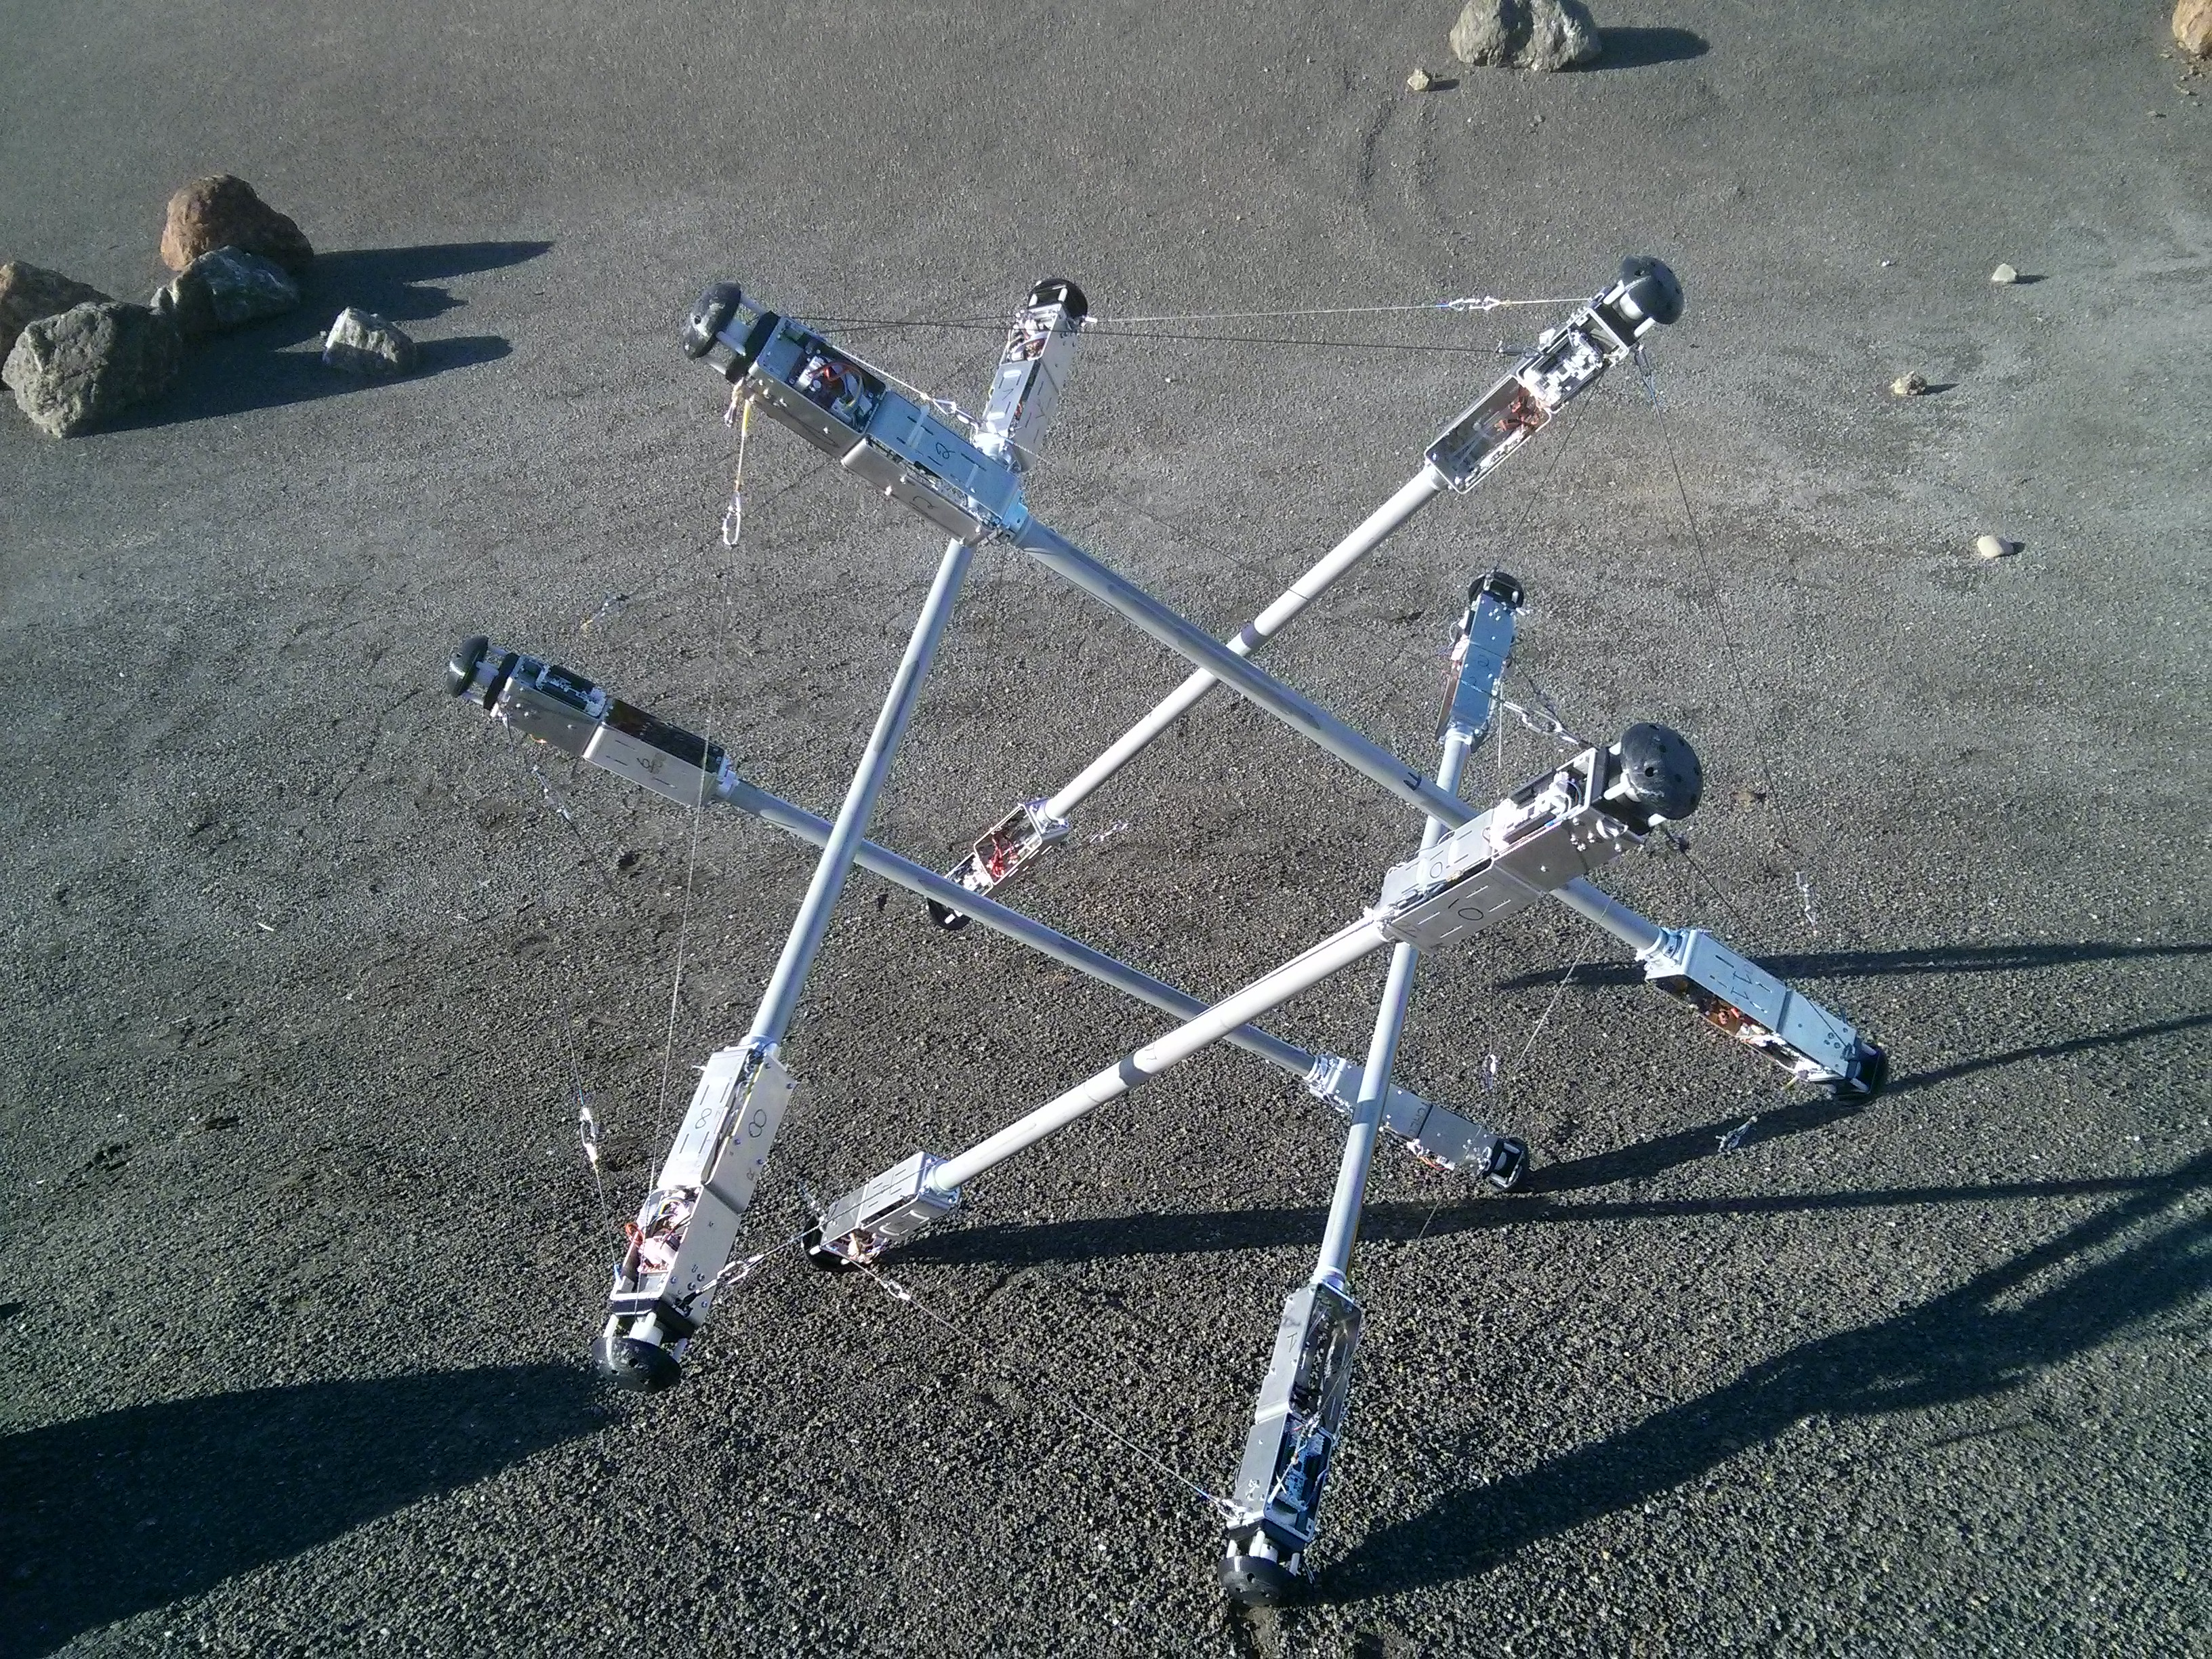
\includegraphics[width=0.8\columnwidth]{tex/img/superball_roverscape2_cropped.jpg}
      \caption{SUPERball, fully assembled, in the NASA Ames Research Center Roverscape.}
      \label{fig:SB}
\end{figure}

As part of our research for the NASA Innovative Advanced
Concepts  (NIAC)  program,  we  are  developing  the \SB{} (Spherical Underactuated Planetary Exploration Robot),
which is a compliant icosahedron tensegrity robot designed
for   planetary   landing   and   exploration, seen in figure \ref{fig:SB}.   Tensegrity   robots
are  soft  machines  which  are  uniquely  able  to  compliantly
absorb  forces  and  interact  with  unstructured  environments.
However, instead of engineering a single new robot, we have
chosen  to  develop  a  fundamentally  reusable  component  for
tensegrity  robots  by  creating  a  modular  robotic  tensegrity
strut which contains an integrated system of power, sensing,
actuation, and communications. The purpose is to enable the
exploration of the wide range of possible tensegrity robotic
morphologies  by  simply  combining  the  robotic  struts  into
new systems.

Though there is much prior work in a variety of theoretical
areas for tensegrities, engineering knowledge of constructing
practical  tensegrity  robots  is  limited.  Since  a  staggering
variety  of  different  tensegrity  structures  can  be  constructed
from  collections  of  simple  sticks  and  strings, we have made it a priority
to develop self-contained robotic tensegrity struts which can
be  used  to  explore  and  build  a  wide  range  of  tensegrity
robots  simply  by  combining  them  into  novel  structures.
Our  designs  are  driven  by  experimental  results  obtained
from  a  previous  prototype,  ReCTeR  (Reservoir  Compliant
Tensegrity Robot) in combination with simulation results of
our validated tensegrity simulator NTRT (NASA Tensegrity
Robotics Toolkit)~\cite{2917079}\cite{Caluwaerts2013rsif}.

In  order  to  develop  SUPERball  from  ReCTeR's  design
limitations as well as our lab’s need for rapid experimentation
of  various  tensegrity  configurations  and  morphologies,  we
came  up  with  a  modular  tensegrity  platform  to  research
large  scale  robotic  tasks;  e.g.  a  tensegrity  planetary  probe
to explore Saturn's moon Titan.
%Our lab obtained design requirements through an iterative
%approach  involving  NTRT  and  ReCTeR.  As  we  validated  our  NTRT  simulator  by  experimental  validation
%with  ReCTeR~\cite{Caluwaerts2013rsif} and can  now  quickly  evaluate  various
Our lab obtained design requirements through an iterative approach with validated our NTRT simulator by experimental comparison with ReCTeR~\cite{Caluwaerts2013rsif}.
We now can quickly  evaluate  various
tensegrity  configurations  in  simulation  to  find  optimal  mechanical  design  goals.  In conjunction with the  NTRT  solver,  we  also
incorporated  results  obtained  with  our  (open  source)  Euler
Lagrange solver based on Skelton's work~\cite{Skelton2009} and measurements on ReCTeR.
The initial design requirements obtained from the NTRT simulations, refined designs after a first prototype build, and how these compare to other tensegrity robotic systems are given in Table \ref{design_req}.


\begin{table*}[ht]
%\begin{minipage}[t][\linewidth]{
\caption{\SB{} and Related Robots Design Overview.} 
\label{design_req}

\begin{center}%
\resizebox{\columnwidth}{!}{%
\begin{tabular}{lrrrcrrrrrrr}
%\hline
&$\bm{l_{strut}}$ & $\bm{\Delta l_{act}}$ & $\bm{k_{passive}}$ & \bf{tethered?} & \bf{control} & $\bm{f_{act}}$ & \bf{\#act.} & \bf{mass} & \bf{sensors} &\bf{actuators} &\bf{ref.} \\ \hline \hline
\bf{Pneumatic}&\SI{.57}{m} & - & - & Y & open loop & \SI{800}{\newton} & \num{24} & \SI{3.3}{\kg}& none & McKibben& \cite{Koizumi2012b} \\
\bf{ReCTeR}&\SI{1}{m} & \SI{0.3}{\metre} & \SI{28.4}{\newton\per\metre} & N & closed loop & \SI{12}{\newton} & \num{6} & \SI{1.1}{\kg} & F, L, IMU & DC & \cite{Caluwaerts2013rsif} \\
\bf{Rapid Proto Kit}&\SI{.69}{m} & \SI{0.005}{\metre} & \SI{1193}{\newton\per\metre} & N & open loop  & $<$\SI{45}{\newton} & \num{24} & \SI{2.7}{\kg}& none & linear DC &\cite{kim2014rapid} \\
\bf{\SB{} 2014}&\SI{1.5}{m} & \SI{0.2}{\metre} & \SI{613}{\newton\per\metre} & N & closed loop & \SI{140}{\newton}  & \num{12} & \SI{9}{\kg}& F, L, $\tau$, IMU & BLDC& \\
\bf{\SB{} 2015}&\SI{1.7}{m} & \SI{0.42}{\metre} & \SI{998}{\newton\per\metre} & N & closed loop & \SI{250}{\newton} & \num{12} & \SI{21}{\kg} & F, L, $\tau$, IMU & BLDC& 
%Tensegrity Kit 
%\SB{} ICRA 2014 &$1.5\mbox{m}$ & $0.26 {\mbox{m}}/{\mbox{s}}$ & $500 \mbox{N}/\mbox{m}$ & $100\mbox{Hz}$ & $3 \mbox{Nm}$ \\
%\SB{} ICRA 2015
%\hline

\end{tabular}
}
\end{center}
\bigskip
\fontsize{10pt}{12pt}\selectfont
The variable $l_{strut}$ indicates the length of a strut, $\Delta l_{act}$ is the nominal spring-cable retraction length in tension, $k_{passive}$ is the linear stiffness coefficient of a passive spring-cable (or active spring-cable if fully actuated), tethered indicates if the robot is powered externally or by internal systems, control indicates whether sensor feedback is used, $f_{act}$ is the nominal actuated spring-cable tension and \#act. is the number of actuators. In the sensors column, F represents a linear force sensor (for cables), L is cable length sensor (in the form of motor encoders), $\tau$ represents a torque sensor for motors, and IMU represents an accelerometer/gyroscope inertial motion sensing unit. Actuators are specified as DC motors or brushless DC (BLDC) motors. The SUPERball 2014 values are revised original design requirements based on NTRT simulations, and changed to the 2015 values after additional detail design. %

\vspace{-0.2cm}

%\end{minipage}
\end{table*}

The work presented here is work verifying our in house tensegrity simulators.
In order to achieve this, the group decided to use a \SB{} like structure with a center payload.
This is believed to be closer to the proposed build profile of a real tensegrity probe, where the main science modules will be contained within the payload.
Protecting this science payload is the main goal for and EDL scenario.
Figure \ref{fig:NTRT_SB} shows a 3-D representation of \SB{} with a payload generated within NTRT.

\begin{figure}[thpb]
      \centering
      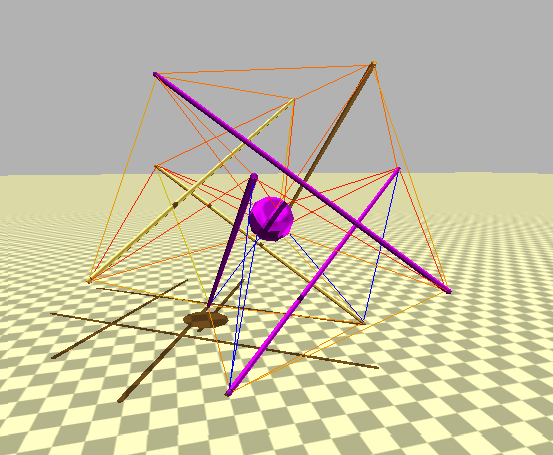
\includegraphics[width=0.8\columnwidth]{tex/img/1.png}
      \caption{SUPERball with a payload modeled within NTRT.}
      \label{fig:NTRT_SB}
\end{figure}

\section{Euler-Lagrange Model}
In order to verify the simulation results produced by our NTRT simulator, we decided to compare the behavior of the NTRT to a published analytic model for tensegrity systems.
We choose to use Skelton's dynamic equations because it is a well accepted and used model.
It may be found in his \emph{Tensegrity Systems} book \cite{skelton_tensegrity_2009} which is based on his work in \cite{skelton2005dynamics}.
In order to solve the dynamic equations with interactions with the environment, an Euler-Lagrange approach is used as well as Skelton's constrained class one structure.
The lagrange equation for a constrained rod is given by
\begin{equation}
\label{eq:lagrange}
L = T - V - c
\end{equation}
where
\begin{align}
\mathbf{b} &= l^{-1}(\mathbf{n}_{j}-\mathbf{n}_{i})\label{eq:normalizedVector}\\
c &= \frac{\mathbf{J}\xi}{2}(\mathbf{b}^{T}\mathbf{b}-1)\label{eq:constraint}
\end{align} 
Equation \eqref{eq:normalizedVector} is the normalized vector of a rod with \(\mathbf{n}_{i,j}\) the nodal positions in \(R^3\), and equation \eqref{eq:constraint} contains the lagrange multiplier \(\xi\) to keep \eqref{eq:normalizedVector} constrained.
\(\mathbf{J}\) is also defined as the inertia matrix for a one dimensional rod in three dimensional space.
In order to define the system of \(k\) rods we need to define a combined Lagrangian as
\begin{equation}
\mathbf{L} = \sum_{i=1}^{k} L_{i}\label{eq:combinedLagrangian}
\end{equation}
where \(L_{i}\) is the Lagrange function for each rod.
Using the approach outlined in Skelton's book for deriving the equations of motion, we can then derive the configuration matrix
\begin{equation}
\mathbf{Q} = \begin{bmatrix}
	\mathbf{R} & \mathbf{B}
	\end{bmatrix}\label{eq:configMatrix}
\end{equation}
where \(\mathbf{R}\) and \(\mathbf{B}\) are matrices containing the translational and rotational vectors, respectively. They have the form
\begin{align}
\mathbf{R} &= \begin{bmatrix}
	\mathbf{r}_{1} & \cdots & \mathbf{r}_{k}
	\end{bmatrix}\label{eq:transR}\\
\mathbf{B} &= \begin{bmatrix}
	\mathbf{b}_{1} & \cdots & \mathbf{b}_{k}
	\end{bmatrix}\label{eq:rotB}
\end{align}
Also using the procedure to derive generalized forces within Skelton's book, the systems's generalized force equations are computed as
\begin{equation}
\mathbf{F}_{\mathbf{Q}} = \begin{bmatrix}
	\mathbf{F}_{\mathbf{R}} & \mathbf{F}_{\mathbf{B}}
	\end{bmatrix}\label{eq:generalizedForce}
\end{equation}
with
\begin{align}
\mathbf{F}_{\mathbf{R}} &= \begin{bmatrix}
	\mathbf{f}_{\mathbf{r}_{1}} & \cdots & \mathbf{f}_{\mathbf{r}_{k}}
	\end{bmatrix}\label{eq:gForceR}\\
\mathbf{F}_{\mathbf{B}} &= \begin{bmatrix}
	\mathbf{f}_{\mathbf{b}_{1}} & \cdots & \mathbf{f}_{\mathbf{b}_{k}}
	\end{bmatrix}\label{eq:gForceB}
\end{align}
Finally, we can define the resulting equations of motion in a compact form as
\begin{equation}
(\ddot{\mathbf{Q}} + \mathbf{Q}\mathbf{\Xi})\mathbf{M} = \mathbf{F}_{\mathbf{Q}}\label{eq:compactForm}
\end{equation}
where
\begin{align}
\mathbf{\Xi} &= diag\begin{bmatrix}
	0,\cdots,0,\xi_{1},\cdots,\xi_{k}
	\end{bmatrix}\label{eq:lagrangeMatrix}\\
\mathbf{M} &= diag\begin{bmatrix}
	m_{1},\cdots,m_{k},J_{1},\cdots,J_{k}
	\end{bmatrix}\label{massMatrix}
\end{align}
This approach was then implemented in Python utilizing a 4th order Runge-Kutta formula for solving the system of ordinary differential equations.  
In order to implement a gravitational field, a force distribution function is applied along the length of each rod and calculated as a nodal force depending on the given density of the rod.
This external force is then applied to the nodes during each time step, simulating a gravitational field.

\section{Detailed Impact Simulations and Cross-Validation Using Two Simulators}
The NTRT simulator is the most general purpose, allowing us to explore control algorithms and complex environmental interactions, but it is an iterative discrete solver that we were concerned might not be providing accurate answers.  The E-L solver, on the other hand, has a much stronger analytical basis and should provide very accurate answers, but is limited because some of the nodes (rod ends) must be constrained and locked into place.  This is unrealistic for the deformation caused during landing, and makes it an inappropriate choice for mobility and controls research.
If ground contact forces are incorporated into the E-L solver and code optimization implemented, it could be used in conjunction with a unscented kalman filter for state estimation propogation.
This tool could then be used to develop online learning algorithms for mobility research.

In this section, we compare the NTRT simulator and E-L solver at the moment of impact with the ground. 
The simulations are compared at the moment of impact with the ground because our implementation of the analytic E-L solver requires select nodes to be constrained.
We setup the structure so that it is barely in contact with the ground and is in balance at time equal to 0. 
In both simulations, we add an initial velocity equal to the terminal velocity of Titan, and compared each vertical trajectory, vertical velocity, and vertical acceleration of the payload. 
Since the structure's horizontal speed is zero at the beginning and the structure is symmetrical, the payload's horizontal components of position, velocity and acceleration are zero. 
As it can be seen in the Figures \ref{fig:vsPosition} and \ref{fig:vsVelocity}, both simulators closely match and generate the same results for position and velocity with the error margin close to zero. 
Comparing the accelerations generated by two simulators (Figure \ref{fig:vsAccelerations}), it can be seen that there is a bigger difference. 
The reason behind this difference is the fact that NTRT uses Bullet, which is a discrete time simulator and accelerations are calculated using two point estimations from velocities at the timestep before.  Yet, even with these differences in accelerations, our conclusion at the end of the comparison is that both simulators showed the same basic dynamics and their results were close enough that we could move forward using the more general purpose NTRT Simulator for our controls, mobility, and landing experiments.


\begin{figure}[htb]
   \centering
   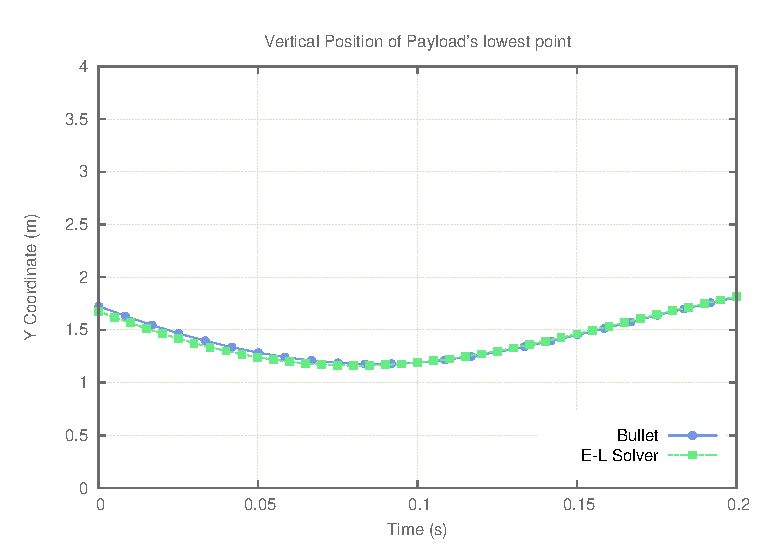
\includegraphics[width=0.8\columnwidth]{tex/images/landing/bulletVsEL/SimVsEL}
   \caption{NTRT vs EL: Vertical Position}
   \label{fig:vsPosition}
\end{figure}

\begin{figure}[htb]
   \centering
   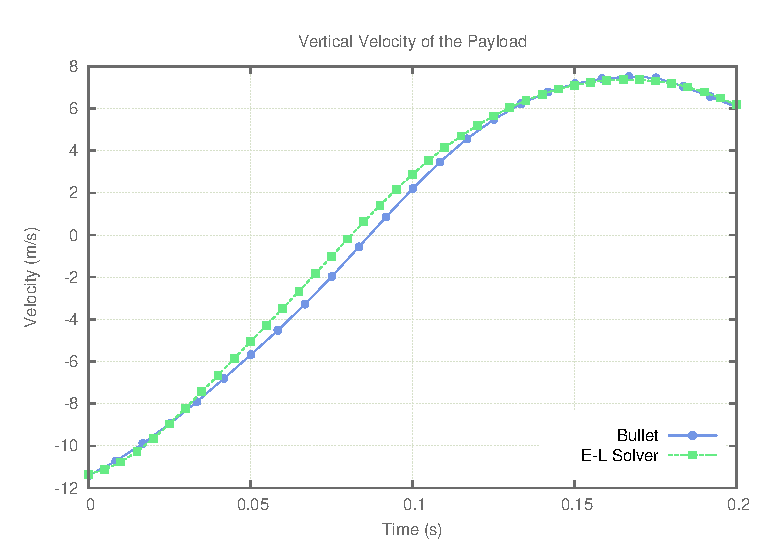
\includegraphics[width=0.8\columnwidth]{tex/images/landing/bulletVsEL/Velocities}
   \caption{NTRT vs EL Vertical Velocity}
   \label{fig:vsVelocity}
\end{figure}
\begin{figure}[htb]
   \centering
   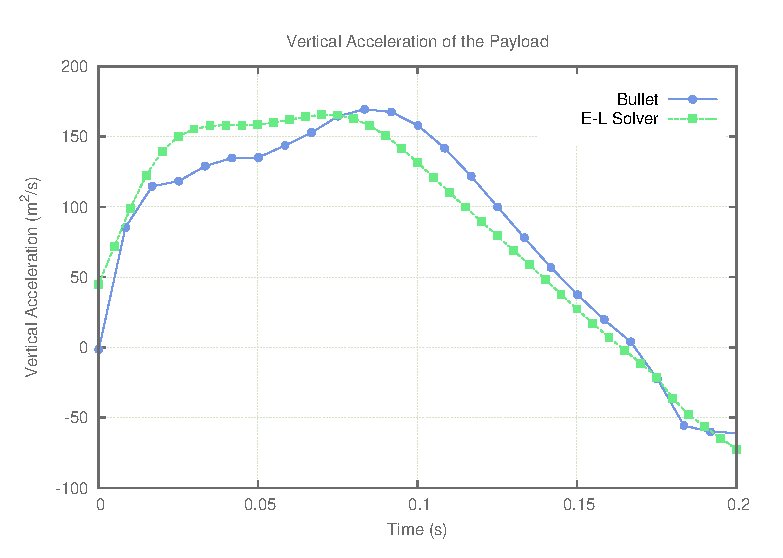
\includegraphics[width=0.8\columnwidth]{tex/images/landing/bulletVsEL/VelocityDerivatives_SimVsEL}
   \caption{NTRT vs EL Vertical Acceleration}
   \label{fig:vsAccelerations}
\end{figure}


\section{Simulated Drop Tests and Payload Protection}

Finally, we performed extensive analysis on drop tests and the protection provided to a payload.   As expected, we found that by varying the rod lengths, which impacts the stroke distance for the payload to decelerate, we could control the maximum deceleration experienced by the payload while ensuring that it did not collide with the ground or structure.  For example, with rods of 1.5 meters in length, our payload experienced a max deceleration of 21.4G when landing at 15 m/s. In figure \ref{fig:rodvsG} we show the results of a series of drop tests with different rod lengths and show the resulting maximum deceleration and forces experienced in the tension members.   As can be seen from these graphs, even for reasonable rod lengths, the maximum G's are acceptable for most instruments, and the maximum forces experienced by the cables are easily within ranges that can be engineered for.  In all tests we kept the total system mass constant, at 100kg (which is 70kg for the payload and 5kg per rod) in order to highlight the impact of structural geometry and rod length.  For the tension members we used spring constants of 44 kN/m for the cables around the perimeter and 10 kN/m for the cables attached to the payload.  Also, the results in Figure \ref{fig:rodvsG} were found using the landing orientation of 35 degrees around X axis and 45 degrees around Z axis, which we selected from our orientation studies discussed below. 

\begin{figure}[htbp]
\centering
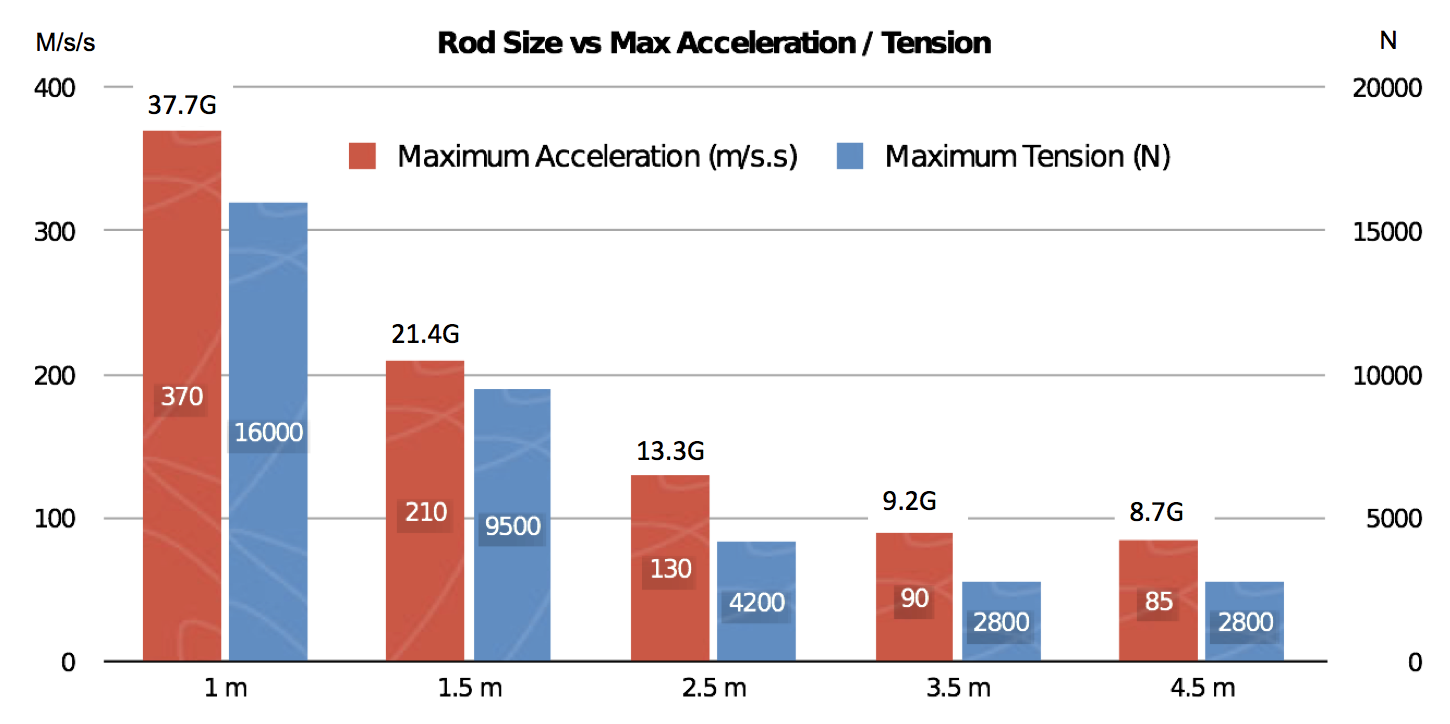
\includegraphics[width=0.8\columnwidth]{tex/images/rodvsG_fixed2}
\caption{{\em {\bf Landing Forces Study}. This shows how rod length impacts maximum deceleration of the payload and  the maximum forces experienced by the tension cables.  All tests were conducted with a landing velocity of 15 m/s onto a hard surface.}}
\label{fig:rodvsG}
\end{figure}

A very interesting point to consider is that the mass of our system will grow in a linear fashion with the length in the rods, while providing increasing payload protection.  On the other hand, the mass of airbags increases with the square of the radius, which is one of the reasons that the MSL rover, with its increased size and mass, had to switch from the airbag approach to the more complex Sky Crane approach.  While this study has focused on small light-weight mission concepts, we expect that there are compelling advantages to scaling up to handle larger payloads and we look forward to studying this further in the future.

\section{Landing Orientation Studies}
In order to study how landing orientation affects payload decelerations and impact events, we conducted a systematic study of landing orientations.  Since we wanted to get meaningful data, even for bad orientations, we used a larger tensegrity with 4 meter rods so the data wouldn't saturate.  Our success criteria for this study was that the decelerations had to stay under an upper limit of 25G deceleration of the payload, and the payload had to avoid collision with the ground or parts of the tensegrity structure.  Figure \ref{fig:landingHeatMapRot} shows the orientations that were safely within these criteria (black) or failed one or both of the criteria (colored).  By using a simple trailing streamer during descent it would be possible to control landing at an optimal orientation and enable the use of smaller structures with shorter rods because the orientation control would maximize the available stroke for the payload to decelerate within the structure.  Conversely, we can use these studies to know what the worst possible landing scenario will be and choose a structure size which will allow safe landing at any orientation.

\begin{figure}[htbp]
   \centering
   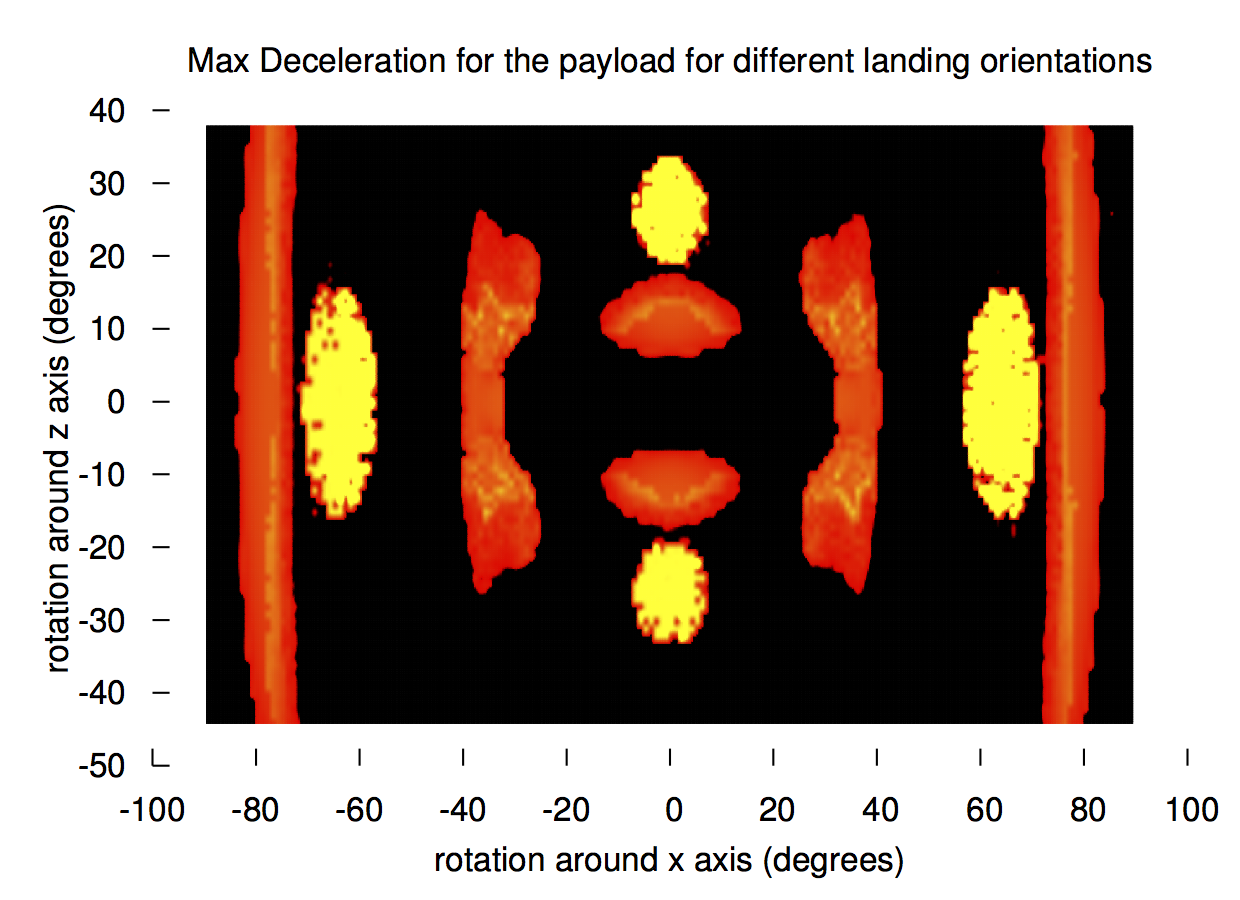
\includegraphics[width=0.8\columnwidth]{tex/images/landing/landingHeatMapRot.png}
   \caption{\em Heat map of the maximum acceleration that the payload encounters for all possible landing orientations. Black areas are safe, colored areas are where the payload does not meet one or both success criteria.}
   \label{fig:landingHeatMapRot}
\end{figure}


\section{Conclusions from Simulation Experiments}
In our landing analysis we developed and cross-validated two different simulation methods that allowed us to explore the capabilities of a tensegrity structure to absorb the forces of landing and to simultaneously protect a delicate payload.  This analysis confirmed that indeed it is possible to do so using a 6-bar tensegrity probe while maintaining maximum decelerations experienced by the instrument-containing payload to forces less than 25G, despite the structure landing at 15 m/s (which is greater than terminal velocity on Titan).   Comparing this to the Huygens probe's landing acceleration of \(32G\) \cite{lorenz1994huygens}, the tensegrtiy probe will have a \(43\% \) reduction in \(G\) forces experienced by the scientific payload, despite the Huygens probe's use of parachutes to land at 1/3 of the speed of our tensegrity probe.

\chapter{Mechatronic Design}

An ideal tensegrity system, either robotic or static, is a collection of rigid compressive elements suspended within a network of tensioned cables. 
For a robotic tensegrities without a payload, the actuation and supporting electronics would be logically designed into the compressive elements. 
Making each compressive element identical will also make the over all design and support of the entire tensegrity robot simplier. 
For SUPERball, each compressive element would be comprised of three parts: two identical end caps and a piece of tube stock. 
The end cap was designed 

\section{Mechanical}
Write about the mechanical design of SUPERball. Make sure to give credit where credit is due.

B.  Mechanical Design
SUPERball  is  an  icosahedron  tensegrity  structure  com-
prised  of  12  motors  at  the  end  of  the  robot’s  6  rods.  Each
rod  is  comprised  of  three  main  elements,  2  modular  end
cap  assemblies  containing  all  the  mechanical  and  electrical
systems   and   a   connecting   aluminum   tube   as   a   support
structure. The main structural elements of the end caps were
kept  simple  and  in  sections  to  enable  each  end  cap  to  be
modular  as  well  as  self  contained  so  that  the  end  cap  may
be removed from the connecting rod as one whole unit. The
end  caps  are  held  onto  the  connecting  rods  by  a  simple
tube  collar  for  easy  removal.  There  are  5  sections  to  the
modular end cap which are, a spring holder, battery holder,
motor and electronics element, cable actuation section, and a
ground contact section. These sections as they are designed
for SUPERball are shown in Fig. 4. Each of these 5 sections
can  be  removed  from  the  rod  as  a  full  sub-assembly  and
replaced with a new component, increasing the versatility of
each rod.
A  lesson  learned  from  ReCTeR  was  that  externally  ex-
posed springs are not ideal for a robotic system. The exposed
springs get caught on objects and the assumption of massless
cables  can  no  longer  be  applied.  On  the  modular  end  cap
for SUPERball, an enclosed compression spring system was
developed  to  alleviate  these  issues.  Compression  springs
were chosen so that during any unknown impact, the springs
would not plastically deform. For SUPERball, a spring with
a spring constant of
613
N=m
is attached to a passive cable
element  and  a
2850
N=m
spring  is  attached  to  an  actuated
cable.  The  passive  spring  has  a  much  higher  compressive
range to allow for pretension to be instated into the passive
springs.  A  working  prototype  of  our  spring  holder  system
can be seen in Fig. 5.

\section{Electrical}
Write about the electronic board used on SUPERball.\\

SUPERball  was  developed  with  distributed  controls  in
mind.  Each  rod  end  cap  houses  two  control  boards,  one
for  motor  driving  and  one  for  handling  sensing  and  com-
munications. Each board hosts a Microchip dsPIC33EP. The
motor driver is a BLDC/PMSM driver board capable of block
commutation and sensorless sinusoidal control. Each sensor
board is equipped with an ADC
(24bit Analog AD7193)
and
9 DOF IMU data
(MPU6000 and MAG3110)
.
Two custom force sensors were developed for the SUPER-
ball, a reaction torque sensor and a compression force sensor.
Fig. 6 shows the reaction torque sensor. It is a symmetrical
four  arm  cross  design  with  the  half  bridge  located  in  the
center of each arm. This sensor, along with the compression
sensors and current sensors allow us to implement high level
control schemes such as impedance control in which the full
state of the mechanical and electrical system must be known.

- Untethered electronics
- 

To this end, we tried to develop electronics which where extensible for various communications
Another driving parameter was the ability to drive the 100W BLDC Maxon motors chosen from the initial iterative design.
These two main design criteria governed our prototype to implement four separate electronic boards per end cap.
Three boards are custom designed PCBs and the fourth is an ARM based computer called Beagle Bone Black.
Each custom PCB is designed for very different purposes: A board to condition sensor data and run real-time control loops, a board to condition and distribute a 5.5V electronic power rail and a 24V motor power rail, and a board to control the 100W BLDC motor. 
The boards are simply named by their main purpose, thus Sensor, Power, and Motor board, respectively.

\subsubsection{Sensor Board}
The sensor board was originally designed as the main processing unit on an end cap for SUPERbal. 
However, the design and building process has lead to the coupling of the sensor board with a Beagle Bone Black.
These two versions are dubbed v1 and v2, respectively.
I will first write about v1 of the sensor board, then follow up on how v2 was changed.\\

The main processing unit on each sensor board is Microchip's dsPIC33EP128GP506, a 16 bit microcomputer running at 140MHz. 
Besides the designer's familiarity with this family of microcomputers, the dsPIC33E chips feature multiple Universal Asynchronous Receiver/Transmitter (UART), Serial Peripheral Interface (SPI), and Inter-Integrated Circuit (I2C) communication modules. 
The dsPIC33E also features an ECAN modules with 2.0B support, a 12 bit Analog to Digital Converter, and four Direct Memory Access (DMA) channels. 
All these moudles coupled with almost complete pin to peripheral pin remapping made the microcomputer a solid choice for our sensor board. 

\section{Communication and Data Flow}




%\input{./tex/Results.tex}
\chapter{Current and Future Work}

\section{\SB{} Current State}
At this point, the first goal proposed in section \ref{goal} has been achieved.
\SB{} is composed of twelve Modular Tensegrity Robots (MTR) attached as the ends of 6 rods connected in a icosahedron geometry, and may be seen in figure \ref{fig:SB}.
Preliminary testing of the system, presented in the following sections, has shown many of the basic functions and features that will enable goals two and three.
All data collected in this section was collected through the wireless ROS network with no extra sensors or equipement apart from what was designed into the system, explained in chapter \ref{design}. 

\subsection{Dynamic Torque Sensor Testing}
\begin{figure}[thpb]
      \centering
      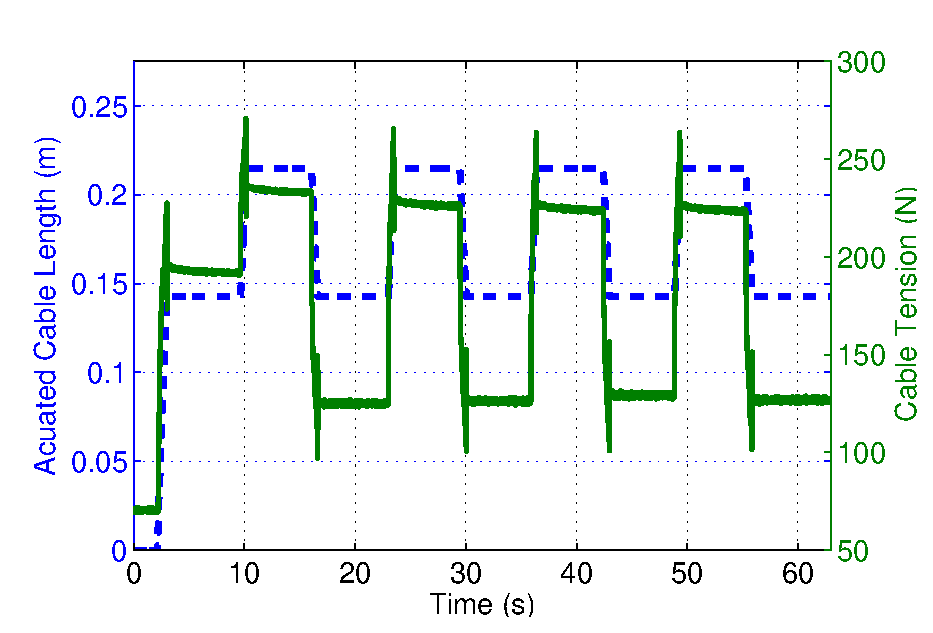
\includegraphics[width=0.8\columnwidth]{tex/img/ICRA2015_dynamic_sensor_test}
      \caption{Motor mount torque sensor data and motor position data recorded during a square wave input position trajectory for a single motor. This plot shows measured tension from the sensor and cable length from motor encoder measurements as a function of time for this dynamic movement.}
      \label{fig:sensor1data}
\end{figure}

This test was performed to demonstrate the force sensors' ability to capture data under dynamic motion.
Figure~\ref{fig:sensor1data} shows a plot of sensor data from one end cap whose motor is commanded in a square-wave position trajectory.
The position trajectory had a period of \SI{13}{\second}, and oscillated between \SI{10}{\radian} and \SI{15}{\radian} of the output shaft measured before the gearbox, by the encoder.
The trajectory of sensor torque values reasonably tracks the position square wave: the commanded position trajectory starts at 10 seconds and ends at 62 seconds, as does the sensed tension square wave.
The overshoot on the torque sensor measurements is due to the system inertia and spring dynamics.

\subsection{Global Force Redistribution Sensor Testing}

\begin{figure}[thpb]
      %\vspace{-0.5cm}
      \centering
      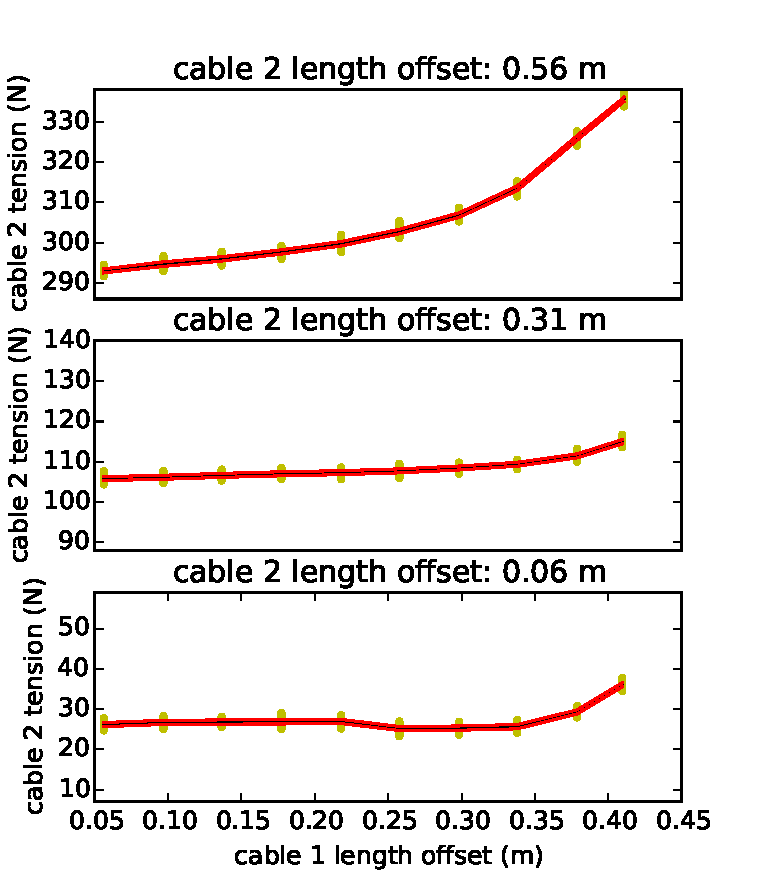
\includegraphics[width=0.55\columnwidth]{tex/img/sensor2_original}
      \caption{Global force redistribution test. Yellow marks are the means of roughly 5,000 tension sensor measurements of \emph{cable 2} opposite that which is actuated (\emph{cable 1}.) The black line shows the linear interpolation between points, with the red boundary as standard deviation. The pretension in the sensed cable is adjusted in each test, showing measurement sequences at increasing pretensions.}
      \label{fig:sensor2data_forcedistribution}
\end{figure}

A test was performed to validate the distribution of tension throughout the system, and to show that all sensors can work in conjunction simultaneously.
Figure~\ref{fig:sensor2data_forcedistribution} shows tension readings from a different motor-mount torque sensor on the opposite side of \SB{} (Cable 2) from a cable which is being retracted (Cable 1.)
Cable 2 was not actively actuated during each test.
For each plot in Figure~\ref{fig:sensor2data_forcedistribution}, the actuated cable was retracted with various step inputs marked in the figure.
Each data point in this figure (yellow) was collected by averaging data from the sensor board for a total of 5 seconds at 1 kHz, after waiting 2 seconds after the step input actuation to avoid dynamic effects.
These tests were done with different levels of pretension on the sensed cable: this pretension was adjusted by changing the length of the sensed cable.
Though the lower-pretension tests show smaller changes in readings, the higher pretensions show increasing readings which demonstrate the ability to sense forces throughout the tension network in pseudo-equilibrium states, as well as \SB{}'s passive force redistribution properties.

\subsection{Basic Locomotion}
\label{basic_locomotion}
Using a basic step input to a single motor, \SB{} can perform a simple transition from one face of the icosahedron to another.
Figure \ref{fig:superball_flop_flat} shows an test where a motor retracts a cable, induing a flop.
The idea of this type of simple transition is to deform the base equilateral triangle such that the center of mass "moves" over the triangle's edge.
The robot becomes unstable and gravity pulls the system over.
The momentum of the system then rolls the robot through the adjacent isosceles triangle to the next equilateral triangle.
In this test, the motor retraction was preset and experimentally derived earlier.

\begin{figure}[t]
    \centering
    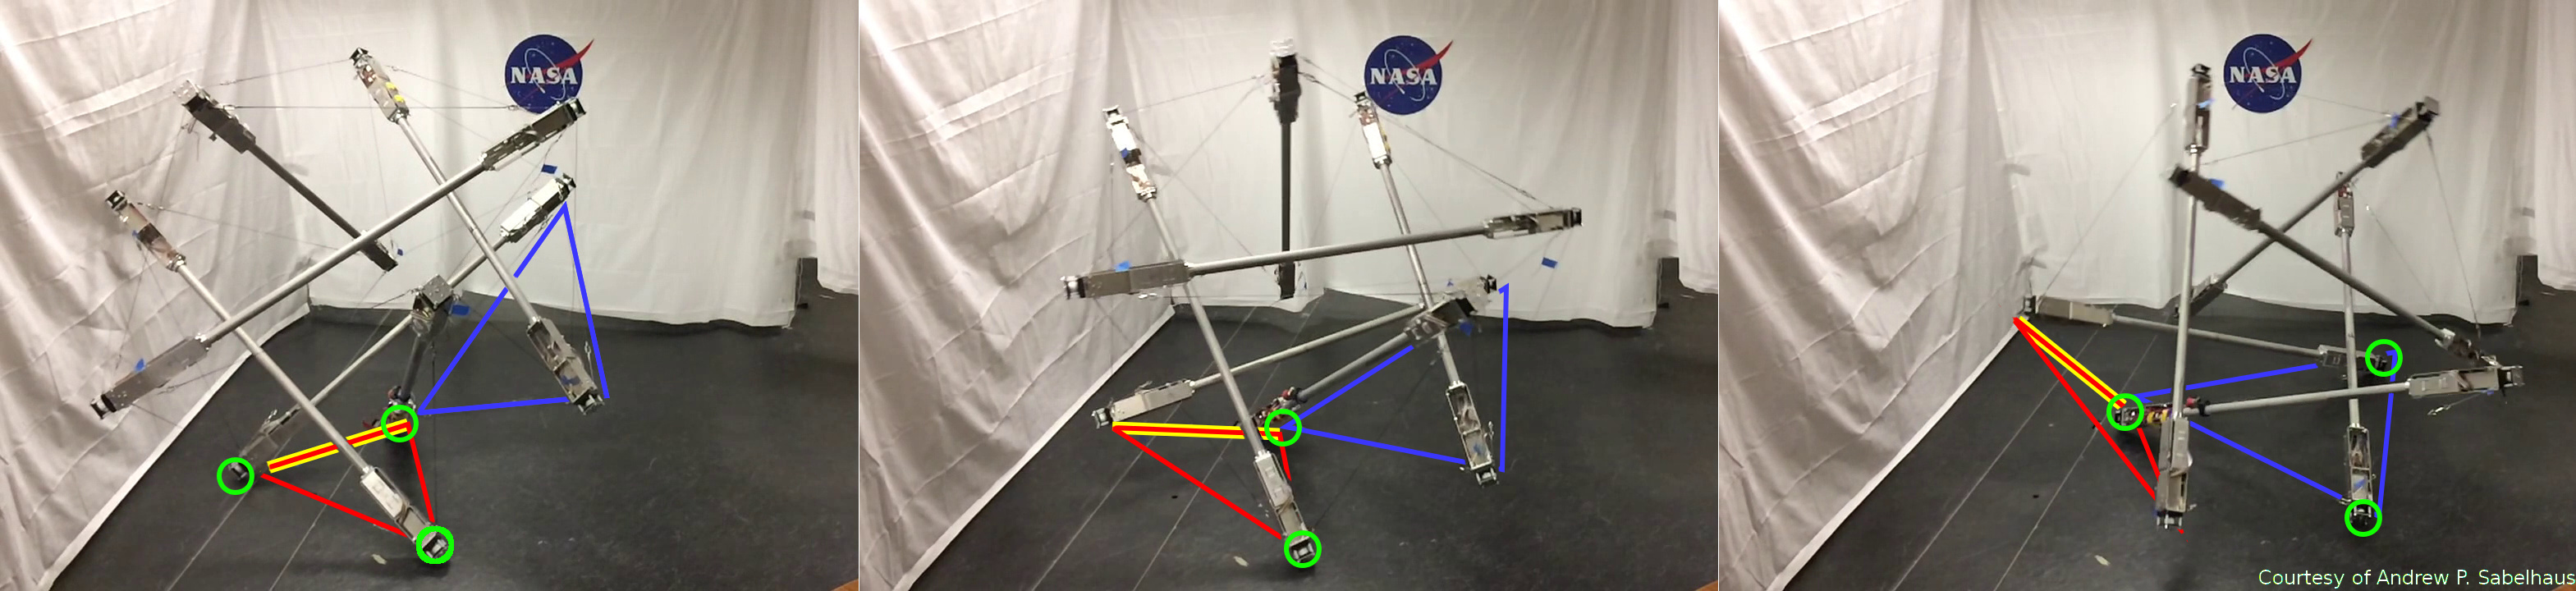
\includegraphics[width=1\linewidth]{tex/img/superball_flop_combined_betterlabels}
    \caption{\SB{} performing a single face-change movement, from one equilateral triangular face to another. The robot begins with all MTRs of the red triangle touching the ground. Then, \SB{} retracts the yellow-highlighted cable on the red triangle, inducing movement. Frame 2 shows \SB{} halfway through the movement with only two points of contact on the ground. Finally, frame 3 shows \SB{} at the end, with all 3 points of the blue triangle in ground contact.}
    \label{fig:superball_flop_flat}
\end{figure}

\section{Future Work}

%\subsection{Proposed Controls Methods}

\subsection{Open Loop Locomotion Control}
\label{open_loop}
For clarity, open loop used here is open in regards to the locomotion system's ability to change robotic motor inputs based on environmental sensing.
Work presented in~\cite{iscen2014flop} shows through simulation that a tensegrity system like \SB{} can achieve a rolling gait by deforming the triangle currently in contact with the ground.
Though \SB{} is not fully actuated (all 24 external cables are attached to motors), a derivative of this work may be able to be applied to \SB{}.
Leveraging the experimental results from section \ref{basic_locomotion}, \SB{} can achieve open loop locomotion quite easily with the addition of detecting which face of the robot is on the ground.
To achieve this ground detection, I propose to use the IMU modules on each sensor board to detect earth's gravity field and/or ground contacts when a rod contacts the ground.
Using a basic machine learning technique, like k-nearest neighbor, may enable successful classification of where the ground is in relation to the robot.

\subsection{Closed Loop Locomotion Control}
There has been preliminary results done by~\cite{burms2015online} which demonstrates a tensegrity robot sensing different enviromental terrains.
This shows promise that a tensegrity robot may sense changes in terrain without the need for extra sensors.
If a similar technique can be achieved on \SB{} in a real-time manor, then the open loop gait pattern used from \ref{open_loop} can be altered to better locomote over the sensed terrain.
This new locomotion gait may either be hand tuned parameters or learned behavior.


% Outline
% Intro about tensegrities. Explain what the structure is and why it is important. Good to mention ideal tensegrities, class system, and prior robots and research.
% Modeling: This section will be a short section on basic linear modeling of a tensegrity structure. Mention that this is not my work, but and explination of prior research. 
% Mechatronics: This will be the longest section. Start off by talking about NIAC and the NASA proposal. Then move to how that directed over arching desgin goals. Move to then talk about the design matrix for SUPERball and how we choose some of the components that we did. Finish by explaining each major portion of the system.
% Results: This section will talk about the itial results from SUPERball. Tension information, motor power and control, battery monitoring, communication (ROS, CAN), 
% Future Work: Talk about where we are taking the project. Movement, learning, etc.

% Bibliography:
\clearpage
\bibliographystyle{plain}
\bibliography{Advancement_Doc_Jonathan_Bruce}

\end{document}
